\subsection{Example \#1: single time series analysis}
\label{S:Example_DISP}
\subsubsection{Data description}
This example uses a synthetic time series that mimics displacement data measured on a bridge (Figure~\ref{fig:DataSummary1}). 
The Figure~\ref{fig:DataSummary1}a shows that data points exist between August 2013 and October 2015.
The timestep in the original data is non-uniform; it varies from 1 hour to 25 hours (see Figure~\ref{fig:DataSummary1}b). 
The most frequent time step  (i.e referent time step, see Section~\ref{SS:NonUniform}) is 1 hour, and there is no missing data (see Figure~\ref{fig:DataSummary1}c).
The time series is stationary with a level, a yearly periodic, a daily periodic patterns and a residual autoregressive pattern.

In this example, we choose to resample the original data in order to have a time step of 6h instead of 1h. 

\begin{figure*}[h]
\centering
\begin{subfigure}{\linewidth}
\centering
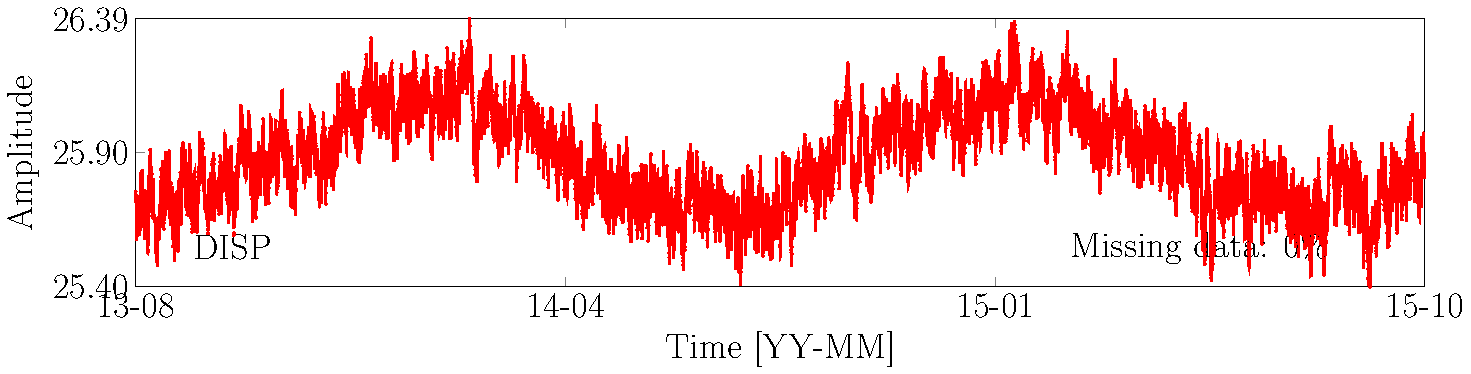
\includegraphics[width=0.9\linewidth]{./docfigs/Example_DISPSIM/raw/ALL_AMPLITUDES.pdf}
\caption{Amplitude}
\end{subfigure}
\begin{subfigure}{\linewidth}
\centering
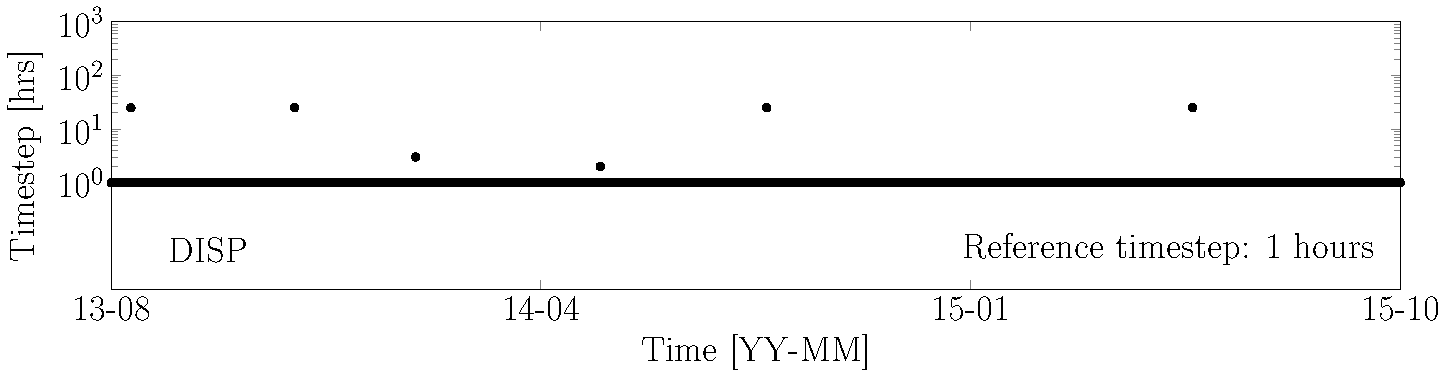
\includegraphics[width=0.9\linewidth]{./docfigs/Example_DISPSIM/raw/ALL_TIMESTEPS.pdf} 
\caption{Timestep}
\end{subfigure}
\begin{subfigure}{\linewidth}
\centering
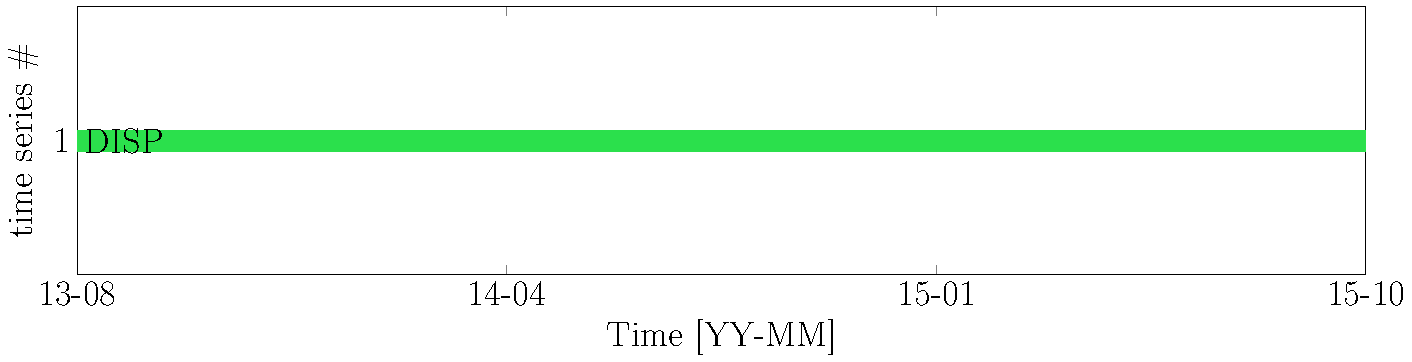
\includegraphics[width=0.9\linewidth]{./docfigs/Example_DISPSIM/raw/AVAILABILITY.pdf}
\caption{Availability}
\end{subfigure}
\caption{Raw data in the example \#1 where the reference timestep is 1h.}
\label{fig:DataSummary1}
\end{figure*}


\subsubsection{Model description}
\label{SS:ModelConstructionExample1}
The model includes one model class, and the hidden states variables are 
\begin{gather*}
\textbf{x}=[x^{\mathtt{LL}}, x^{\mathtt{P1}\text{,yearly}}, x^{\mathtt{P2}\text{,yearly}}, x^{\mathtt{P1}\text{,daily}}, x^{\mathtt{P2}\text{,daily}}, x^{\mathtt{AR}}].
\end{gather*}
The associated model parameters are
\begin{gather*}
\bm\theta=[\sigma_{w}^{\mathtt{LL}}, p^{\mathtt{P}, \text{yearly}}, \sigma_{w}^{\mathtt{P}, \text{yearly}} , p^{\mathtt{P}, \text{daily}}, \sigma_{w}^{\mathtt{P}, \text{daily}}, \phi^{\mathtt{AR}}, \sigma_{w}^{\mathtt{AR}}, \sigma_{v}].
\end{gather*}
The optimized model parameters values computed using the Newton-Raphson algorithm (see~\ref{SS:THModelParameterEstimation}) with a training period of 180 days  are
\begin{gather*}
\bm\theta^{\text{*}}=[0, 365.2422, 0, 1, 0, 0.903, 0.035, 7.8\times10^{-6} ].
\end{gather*}
The optimized initial hidden states mean and covariance values are 
\begin{align*}
\bm \mu^{*}_{0} & = [	25.9,-0.202,-0.004	,-0.004,0.054,-0.012]^{\intercal}, \text{and} \\
\bm\Sigma^{*}_{0} & = \text{diag}([4.21\times10^{-5},	8.3\times10^{-5},	8.46\times10^{-5},	4.29\times10^{-7},	4.29\times10^{-7},	1.59\times10^{-3}   ]).
 \end{align*}
The hidden states computed using the estimated model parameters and initial hidden states are presented in Figure~\ref{fig:Example_DISPSIMOptimizedOptimizedExample1}.

\begin{figure*}[h!]
\begin{center}
\begin{subfigure}{\linewidth}
\centering
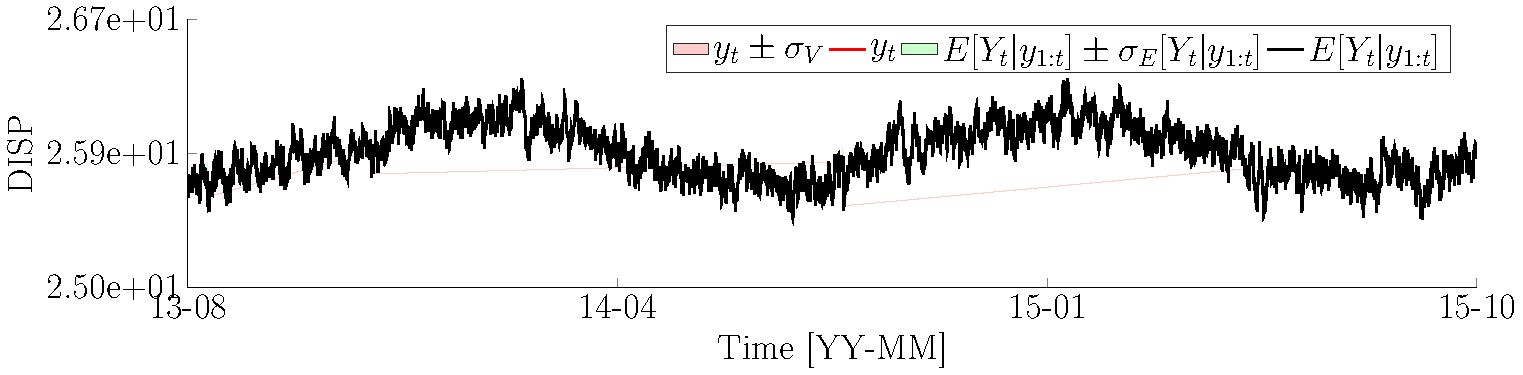
\includegraphics[width=0.9\linewidth]{./docfigs/Example_DISPSIM/optim_param_optim_initialhiddenstate/DISP_ObservedPredicted.pdf} 
\caption{Observed and estimated displacement data}
\end{subfigure}
\begin{subfigure}{\linewidth}
\centering
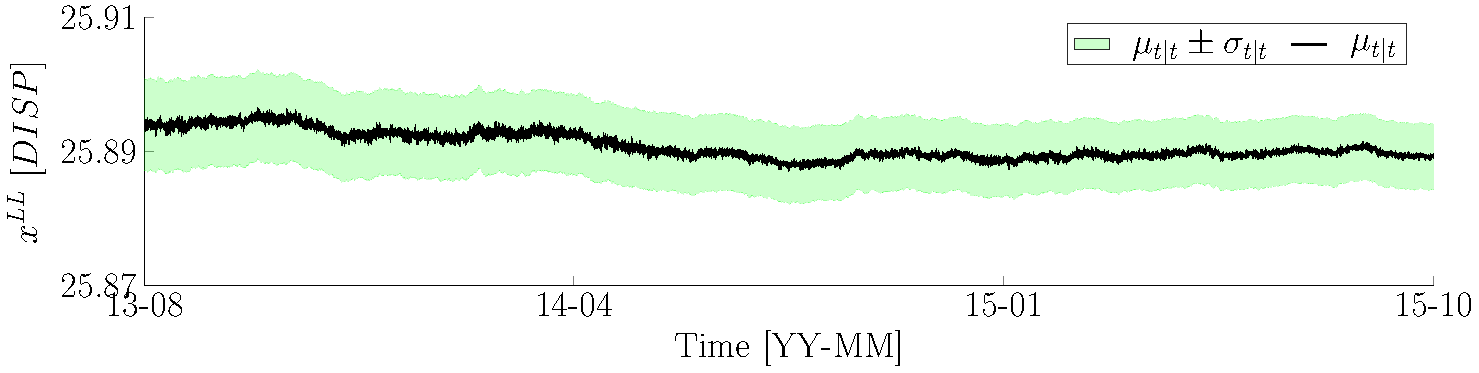
\includegraphics[width=0.9\linewidth]{./docfigs/Example_DISPSIM/optim_param_optim_initialhiddenstate/DISP_LL_1.pdf}
\caption{Estimated displacement local level component.}
\end{subfigure}
\begin{subfigure}{\linewidth}
\centering
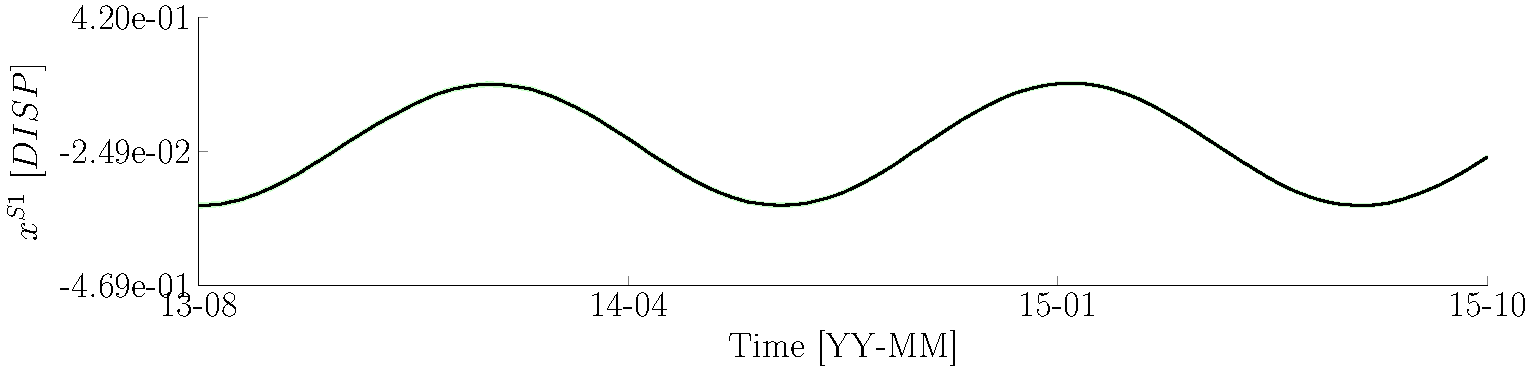
\includegraphics[width=0.9\linewidth]{./docfigs/Example_DISPSIM/optim_param_optim_initialhiddenstate/DISP_S1_2.pdf} 
\caption{Estimated displacement yearly periodic component (first hidden state)}
\end{subfigure}
\begin{subfigure}{\linewidth}
\centering
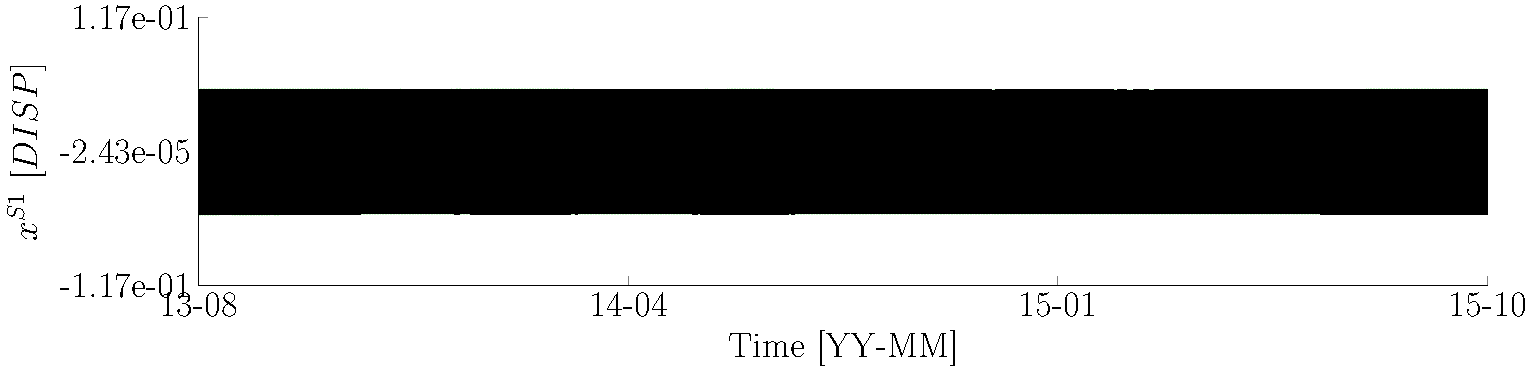
\includegraphics[width=0.9\linewidth]{./docfigs/Example_DISPSIM/optim_param_optim_initialhiddenstate/DISP_S1_4.pdf}
\caption{Estimated displacement daily periodic component (first hidden state)}
\end{subfigure}
\begin{subfigure}{\linewidth}
\centering
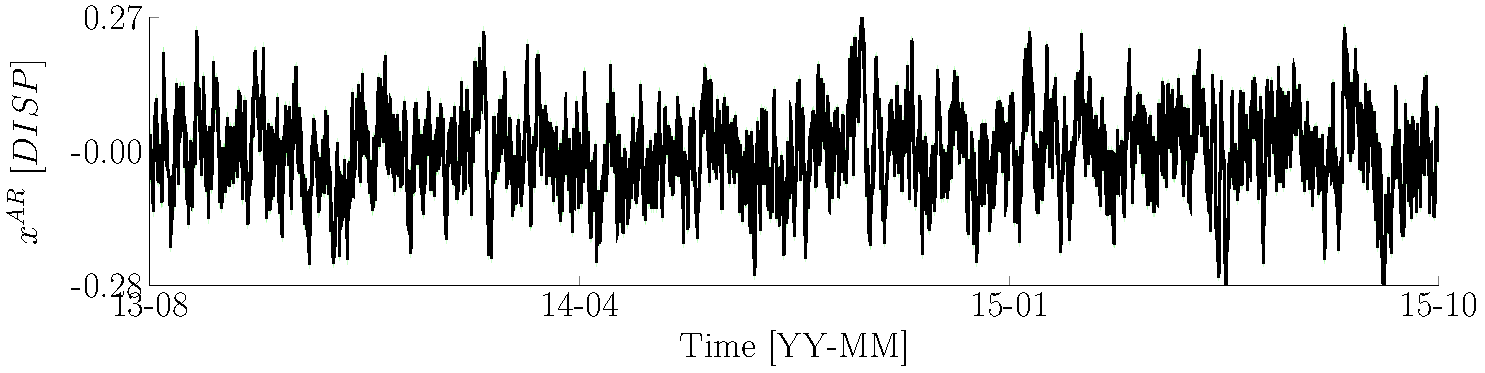
\includegraphics[width=0.9\linewidth]{./docfigs/Example_DISPSIM/optim_param_optim_initialhiddenstate/DISP_AR_6.pdf} 
\caption{Estimated displacement autoregressive component}
\end{subfigure}
\caption{Estimated results using OpenBDLM optimized model parameters and optimized initial hidden states. The hidden states are estimated from the data presented in Figure~\ref{fig:DataSummary1}a. The solid line and shaded area represent the mean and standard deviation of the estimated hidden states, respectively.}
\label{fig:Example_DISPSIMOptimizedOptimizedExample1}
\end{center}
\end{figure*}



\subsubsection{Run the example from pre-existing configuration file}
\label{SS:LoadConfigFileEx1}
There is a configuration file CFG\_Example\_DISP\_optim.m which is located in the ``config\_files'' folder of the OpenBDLM package.
CFG\_Example\_DISP\_optim.m contains the optimized model parameters and optimized initial hidden states values (see Listing~\ref{LST:CFGFileExample1}).
There is also a data file DATA\_Example\_DISP\_optim.mat that is located in the ``data/mat'' subfolder.
Therefore, it is possible to run the example \#1 by following the steps below while interacting with the \MATLAB{} command line:
\begin{enumerate}
\item Start OpenBDLM. Type \colorbox{light-gray}{\lstinline[basicstyle = \mlttfamily \small, backgroundcolor = \color{light-gray}]!OpenBDLM_main('CFG_Example_DISP_optim.m');!}.
\item Access hidden states estimation menu. Type \colorbox{light-gray}{\lstinline[basicstyle = \mlttfamily \small, backgroundcolor = \color{light-gray}]!3!}.
\item Run the Kalman filter to estimate the hidden states. Type \colorbox{light-gray}{\lstinline[basicstyle = \mlttfamily \small, backgroundcolor = \color{light-gray}]!1!}.
\item Save and quit. Type \colorbox{light-gray}{\lstinline[basicstyle = \mlttfamily \small, backgroundcolor = \color{light-gray}]!Q!}.
\end{enumerate}


\begin{lstlisting}[linewidth=\linewidth, style=Matlab-editor,  basicstyle = \mlttfamily \tiny, backgroundcolor = \color{matlab-yellow}, caption = {Configuration file for the example \#1}, label=LST:CFGFileExample1, captionpos=b, float=h!]
%                    OpenBDLM configuration file                          
%          Autogenerated by OpenBDLM on 22-Nov-2018 17:18:09              
%
%% A - Project name
misc.ProjectName='Example_DISP_optim';

%% B - Data
dat=load('DATA_Example_DISP_optim.mat'); 
data.values=dat.values;
data.timestamps=dat.timestamps;
data.labels={'DISP'};

%% C - Model structure 

% Model components
% Model 1
model.components.block{1}={[11 31 31 41] };

% Model component constrains | Take the same  parameter as model class #1
 
% Model inter-components dependence | {[components form dataset_i depends on components from  dataset_j]_i,[...]}
model.components.ic={[ ] };
%
%% D - Model parameters 
model.param_properties={
     % #1       #2       #3    #4    #5         #6       #7     #8     #9    #10
     % Param name Block name  Model Obs Bound Prior Mean Std Values Ref
     '\sigma_w', 'LL',  '1',   '1', [NaN  NaN],    'N/A',  NaN, NaN,   0,         1 %#1   
     'p',        'PD1', '1',   '1', [NaN  NaN],    'N/A',  NaN, NaN,   365.24,    2 %#2   
     '\sigma_w', 'PD1', '1',   '1', [NaN  NaN],    'N/A',  NaN, NaN,   0,         3 %#3   
     'p',        'PD2', '1',   '1', [NaN  NaN],    'N/A',  NaN, NaN,   1,         4 %#4   
     '\sigma_w', 'PD2', '1',   '1', [NaN  NaN],    'N/A',  NaN, NaN,   0,         5 %#5   
     '\phi',     'AR',  '1',   '1', [0  1],        'N/A',  NaN, NaN,   0.903,     6 %#6   
     '\sigma_w', 'AR',  '1',   '1', [0  Inf],      'N/A',  NaN, NaN,   0.035,     7 %#7   
     '\sigma_v', '',    '1',   '1', [0  Inf],      'N/A',  NaN, NaN,   7.8e-06,   8 %#8   
};

%% E - Initial states values 
% Initial hidden states mean for model 1:
model.initX{ 1 }=[	25.9  	-0.202	-0.00406	-0.00439	0.0548	-0.0129  ]';

% Initial hidden states variance for model 1: 
model.initV{ 1 }=diag([ 	4.21E-05	8.3E-05	8.46E-05	4.29E-07	4.29E-07	0.00159 ]);

% Initial probability for model 1
model.initS{1}=[1     ];

\end{lstlisting}



\subsubsection{Run the example from command line interaction}

The analysis of a new dataset usually requires to start from scratch.
This section explains how to run the example \#1 from scratch, that is, how to load the data presented in Figure~\ref{fig:DataSummary1}, configure the model, estimate the model parameters and estimate the hidden states as presented in Figure~\ref{fig:Example_DISPSIMOptimizedOptimizedExample1}.
This may be done by following steps below while interacting with the \MATLAB{} command line
\begin{enumerate}
\item Start OpenBDLM. Type \colorbox{light-gray}{\lstinline[basicstyle = \mlttfamily \small, backgroundcolor = \color{light-gray}]!OpenBDLM_main;!}.
\item Choose the interactive tool. Type \colorbox{light-gray}{\lstinline[basicstyle = \mlttfamily \small, backgroundcolor = \color{light-gray}]!0!}.
\item Enter the project name. Type \colorbox{light-gray}{\lstinline[basicstyle = \mlttfamily \small, backgroundcolor = \color{light-gray}]!Example_DISP!}. 
\item Disregard generating synthetic data. Type \colorbox{light-gray}{\lstinline[basicstyle = \mlttfamily \small, backgroundcolor = \color{light-gray}]!no!}. 
\item Load new data. Type \colorbox{light-gray}{\lstinline[basicstyle = \mlttfamily \small, backgroundcolor = \color{light-gray}]!0!}.
\item Select from the graphical user interface\footnote{Douglas M. Schwarz, 2007, uipickfiles \url{https://www.mathworks.com/matlabcentral/fileexchange/10867-uipickfiles-uigetfile-on-steroids}} the data file Example\_DISP\_DISP.csv located in the folder ``/data/csv/Example\_DISP''. See Figure~\ref{fig:DataLoadingUIPickFileExample1}. The Figure~\ref{fig:DataSummary1} that represents the raw data should popup on screen.

\item Access the resampling menu. Type \colorbox{light-gray}{\lstinline[basicstyle = \mlttfamily \small, backgroundcolor = \color{light-gray}]!4!}. 

\item Resample data to obtain timesteps of 6h (0.25 day). Type \colorbox{light-gray}{\lstinline[basicstyle = \mlttfamily \small, backgroundcolor = \color{light-gray}]!0.25!}. The Figure~\ref{fig:DataSummary1} should popup on the screen this time for the resampled data.

\item Save and continue. Type \colorbox{light-gray}{\lstinline[basicstyle = \mlttfamily \small, backgroundcolor = \color{light-gray}]!7!}. The same figures should popup on the screen again.

\item Select the number of model classes. Type \colorbox{light-gray}{\lstinline[basicstyle = \mlttfamily \small, backgroundcolor = \color{light-gray}]!1!}. 
\item Select the model block components. Type \colorbox{light-gray}{\lstinline[basicstyle = \mlttfamily \small, backgroundcolor = \color{light-gray}]![11 31 31 41]!}.

\item Access the training period modification menu. Type \colorbox{light-gray}{\lstinline[basicstyle = \mlttfamily \small, backgroundcolor = \color{light-gray}]!13!}. 

\item Modify the training period. Type \colorbox{light-gray}{\lstinline[basicstyle = \mlttfamily \small, backgroundcolor = \color{light-gray}]!1!}. 

\item Choose the starting time (day). Type \colorbox{light-gray}{\lstinline[basicstyle = \mlttfamily \small, backgroundcolor = \color{light-gray}]!1!}. 

\item Choose the end time (day). Type \colorbox{light-gray}{\lstinline[basicstyle = \mlttfamily \small, backgroundcolor = \color{light-gray}]!180!}. 

\item Access model parameter estimation menu. Type \colorbox{light-gray}{\lstinline[basicstyle = \mlttfamily \small, backgroundcolor = \color{light-gray}]!1!}. 
\item Start Newton-Raphson algorithm. Type \colorbox{light-gray}{\lstinline[basicstyle = \mlttfamily \small, backgroundcolor = \color{light-gray}]!1!}. Once the algorithm has converged, the optimized model parameters values should be close to the values presented in Section~\ref{SS:ModelConstructionExample1}. Note that it is possible to get slightly different value of parameters with the same performance\footnote{Keep in mind that the optimization may take several minutes to several hours. It is possible to abort the analysis here and to load the configuration file called CFG\_Example\_DISP\_optim.m to load pre-computed values of model parameters, as presented in Section~\ref{SS:LoadConfigFileEx1}.}.
\item Estimate the initial hidden states values. Type \colorbox{light-gray}{\lstinline[basicstyle = \mlttfamily \small, backgroundcolor = \color{light-gray}]!2!}.
\item Access hidden states estimation menu. Type \colorbox{light-gray}{\lstinline[basicstyle = \mlttfamily \small, backgroundcolor = \color{light-gray}]!3!}. 
\item Estimate the filtered hidden states. Type \colorbox{light-gray}{\lstinline[basicstyle = \mlttfamily \small, backgroundcolor = \color{light-gray}]!1!}. The estimation should be similar to the results presented in Figure~\ref{fig:Example_DISPSIMOptimizedOptimizedExample1}.
\item Access export menu. Type \colorbox{light-gray}{\lstinline[basicstyle = \mlttfamily \small, backgroundcolor = \color{light-gray}]!17!}. 
\item Export the current project in a configuration file. Type \colorbox{light-gray}{\lstinline[basicstyle = \mlttfamily \small, backgroundcolor = \color{light-gray}]!1!}.
\item Save and quit OpenBDLM. Type \colorbox{light-gray}{\lstinline[basicstyle = \mlttfamily \small, backgroundcolor = \color{light-gray}]!Q!}.
\end{enumerate}


\begin{figure*}[h]
\begin{center}
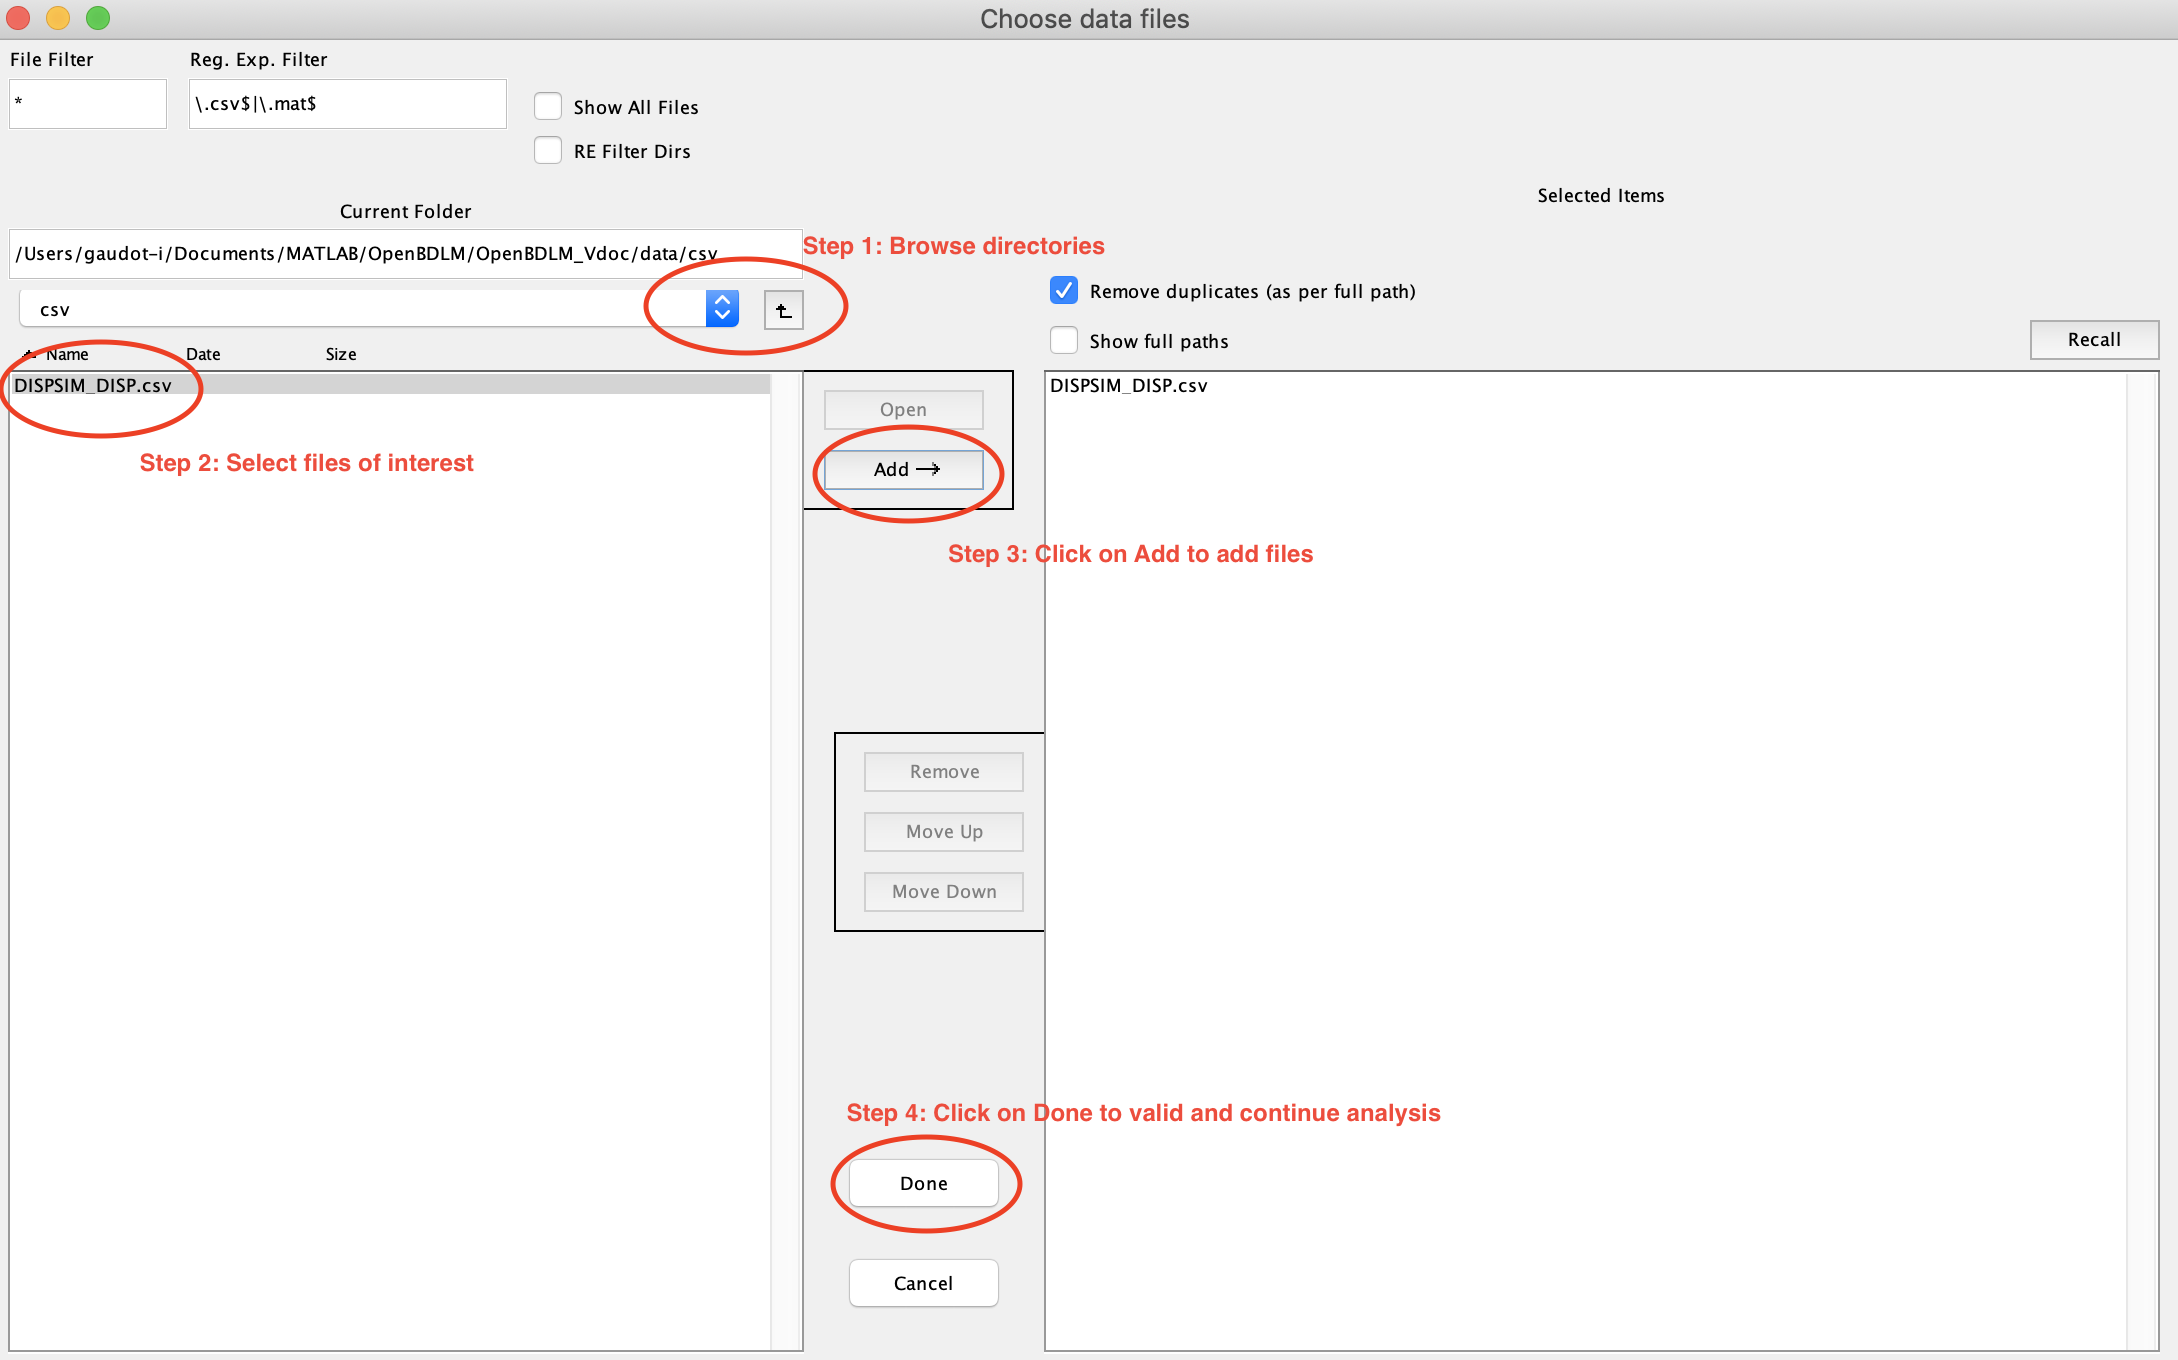
\includegraphics[width=0.9\linewidth]{./docfigs/Example_DISPSIM/dataloading_DISPSIM_uipickfiles_annoted.png}
\caption{Interactive data loading using the graphical user interface.}.
\label{fig:DataLoadingUIPickFileExample1}
\end{center}
\end{figure*}




%\subsection{Step 3: edit and pre-process the data}
%
%The data editing and preprocessing menu as depicted in Listing~\ref{LST:Editing_menu} appear.
%In this example, the objective is to use the data as such.
%Therefore, no editing or preprocessing is done.
%Therefore, type \colorbox{light-gray}{\lstinline[basicstyle = \mlttfamily \small, backgroundcolor = \color{light-gray}]!7!} to save the data as such, and continue analysis.
%
%\subsection{Step 4: configure the model}
%
%First, the program requests the number of model class.
%In this example, the time series data looks stationary and we are not interested in anomaly detection, so type type \colorbox{light-gray}{\lstinline[basicstyle = \mlttfamily \small, backgroundcolor = \color{light-gray}]!1!}.
%Secondly, OpenBDLM asks for the type of block component. 
%Type \colorbox{light-gray}{\lstinline[basicstyle = \mlttfamily \small, backgroundcolor = \color{light-gray}]![11 31 31 41]!} to define a model with a local level, a yearly periodic component, a daily periodic component and an autoregressive component.
%The  output on \MATLAB{} command window during interactive model configuration is presented in Listing~\ref{LST:OpenBDLMModelConfigureExample1}.
%%Press the enter key $\dlsh$ to valid.
%The model is then built, a {\lstinline[basicstyle = \mlttfamily \small, backgroundcolor = \color{light-gray}]!DATA_Example_DISP.mat!} binary data file, a {\lstinline[basicstyle = \mlttfamily \small, backgroundcolor = \color{light-gray}]!CFG_Example_DISP.m!} configuration file, as well as a {\lstinline[basicstyle = \mlttfamily \small, backgroundcolor = \color{light-gray}]!PROJ_Example_DISP.mat!} project file are created.
%The OpenBLDM main menu must appear on the \MATLAB{} command window (see Listing~\ref{LST:OpenBDLMMainMenu}).
%Type \colorbox{light-gray}{\lstinline[basicstyle = \mlttfamily \small, backgroundcolor = \color{light-gray}]!Q!} to save and quit.
%
% \begin{lstlisting}[ frame = single, basicstyle = \mlttfamily \small, caption = { \MATLAB{} command window output during interactive model configuration.}, label = LST:OpenBDLMModelConfigureExample1,  float =h, linewidth=\linewidth, captionpos=b]
%- How many model classes do you want for each time series? 
%     choice >> 1
%     
%     --------------------------------------------------------
%     BDLM Component reference numbers
%     --------------------------------------------------------
%     11: Local level 
%     12: Local trend 
%     13: Local acceleration 
%     21: Local level compatible with local trend 
%     22: Local level compatible with local acceleration 
%     23: Local trend compatible with local acceleration 
%     31: Periodic 
%     41: Autoregressive process (AR(1)) 
%     51: Kernel regression 
%     61: Level Intervention 
%     --------------------------------------------------------
%
%- Identify components for time series #1; e.g. [11 31 41]
%     choice >> [11 31 31 41]
%
%     Building model...
%     Saving project...
%     Project saved in saved_projects/PROJ_Example_DISP.mat. 
%     Printing configuration file...
%     Saving data...
%
%     Database saved in data/mat/DATA_Example_DISP.mat 
%     Configuration file saved in config_files/CFG_Example_DISP.m. 
%
%\end{lstlisting}
%
%
%\subsection{Step 5: open the configuration file}
%
%After the data loading and the model configuration, a configuration file named \lstinline[basicstyle = \mlttfamily \small, backgroundcolor = \color{light-gray}]!CFG_Example_DISP.csv! is automatically created and saved in ``config\_files'' folder.
%Open the configuration file from \MATLAB{} command line by typing  \colorbox{light-gray}{\lstinline[basicstyle = \mlttfamily \small, backgroundcolor = \color{light-gray}]!edit CFG_Example_DISP.m!}.
%The first part of this configuration file as it should appear on the \MATLAB{} editor is shown in Listing~\ref{LST:CFGFileExample1}.
%The Model parameters section of the configuration file shows that the model totalizes 8 model parameters, that is 
%\begin{gather*}
%\bm\theta=\{\sigma_{w}^{LL}, p^{\text{PD1}}, \sigma_{w}^{\text{PD1}} , p^{\text{PD2}}, \sigma_{w}^{\text{PD2}}, \phi^{AR}, \sigma_{w}^{AR}, \sigma_{v}\}.
%\end{gather*}
%%The default value of the model parameters are assigned   using heuristic knowledge or computed from the data using statistics on the data.
%The default model parameters values are 
%\begin{gather*}
%\bm\theta^{\text{default}}=\{0, 365.2422, 0, 1, 0, 0.75, 0.0174, 0.0087002 \}.
%\end{gather*}
%%In the same manner, default value for the initial hidden states are assigned using heuristic knowledge or computed using statistics on the data.
%The default  hidden states mean  and covariance values are 
%\begin{align*}
%\bm \mu^{\text{default}}_{0} & = [25.8 , 5  ,   	0     ,	5   ,  	0    , 	0     ]^{\intercal}, \text{and} \\
% \text{diag}(\bm\Sigma^{\text{default}}_{0}) & = [	0.121 	,0.121 ,	0.121 ,	0.121 ,	0.121 	, 0.0303     ], 
% \end{align*}
% respectively.
%
%\begin{lstlisting}[linewidth=\linewidth, style=Matlab-editor,  basicstyle = \mlttfamily \scriptsize, backgroundcolor = \color{matlab-yellow}, caption = {Example of a configuration file}, label=LST:CFGFileExample1, captionpos=b, float=h!]
%%                    OpenBDLM configuration file                          
%%          Autogenerated by OpenBDLM on 22-Nov-2018 17:18:09              
%%
%%% A - Project name
%misc.ProjectName='Example_DISP';
%
%%% B - Data
%dat=load('DATA_Example_DISP.mat'); 
%data.values=dat.values;
%data.timestamps=dat.timestamps;
%data.labels={'Example_DISP'};
%
%%% C - Model structure 
%
%% Model components
%% Model 1
%model.components.block{1}={[11 31 31 41] };
%
%% Model component constrains | Take the same  parameter as model class #1
% 
%% Model inter-components dependence | {[components form dataset_i depends on components from  dataset_j]_i,[...]}
%model.components.ic={[ ] };
%%
%%% D - Model parameters 
%model.param_properties={
%     % #1       #2       #3    #4    #5         #6       #7     #8     #9    #10
%     % Param name Block name  Model Obs Bound Prior Mean Std Values Ref
%     '\sigma_w', 'LL',  '1',   '1', [NaN  NaN],    'N/A',  NaN, NaN,  0,          1 %#1   
%     'p',        'PD1', '1',   '1', [NaN  NaN],    'N/A',  NaN, NaN, 365.24,      2 %#2   
%     '\sigma_w', 'PD1', '1',   '1', [NaN  NaN],    'N/A',  NaN, NaN,   0,         3 %#3   
%     'p',        'PD2', '1',   '1', [NaN  NaN],    'N/A',  NaN, NaN,   1,         4 %#4   
%     '\sigma_w', 'PD2', '1',   '1', [NaN  NaN],    'N/A',  NaN, NaN,   0,         5 %#5   
%     '\phi',     'AR',  '1',   '1', [0  1],        'N/A',  NaN, NaN,   0.97,      6 %#6   
%     '\sigma_w', 'AR',  '1',   '1', [0  Inf],      'N/A',  NaN, NaN,   0.0192,    7 %#7   
%     '\sigma_v', '',    '1',   '1', [0  Inf],      'N/A',  NaN, NaN,   7.425e-07, 8 %#8   
%};
%
%%% E - Initial states values 
%% Initial hidden states mean for model 1:
%model.initX{ 1 }=[	25.89 	-0.202	-0.00305	0.0331	0.051 	-0.00843   ]';
%
%% Initial hidden states variance for model 1: 
%model.initV{ 1 }=diag([ 3.74E-05	6.85E-05	6.99E-05	5.73E-07	5.73E-07	0.000485	 ]);
%
%% Initial probability for model 1
%model.initS{1}=[1     ];
%
%\end{lstlisting}
%
%\subsection{Step 6: estimate the hidden states}
%
%Type \colorbox{light-gray}{\lstinline[basicstyle = \mlttfamily \small, backgroundcolor = \color{light-gray}]!OpenBDLM_main('CFG_Example_DISP.m');!} in the \MATLAB{} command line.
%Once, the main menu appears, type  \colorbox{light-gray}{\lstinline[basicstyle = \mlttfamily \small, backgroundcolor = \color{light-gray}]!3!}, then \colorbox{light-gray}{\lstinline[basicstyle = \mlttfamily \small, backgroundcolor = \color{light-gray}]!1!} to estimate the filtered hidden states using the default model parameters and default initial hidden states values.
%The value of the log-likelihood is $36626$, and the estimated hidden states are presented in Figure~\ref{fig:Example_DISPSIMDefaultDefaultExample1}.
%
%\begin{figure*}[h!]
%\centering
%\begin{subfigure}{\linewidth}
%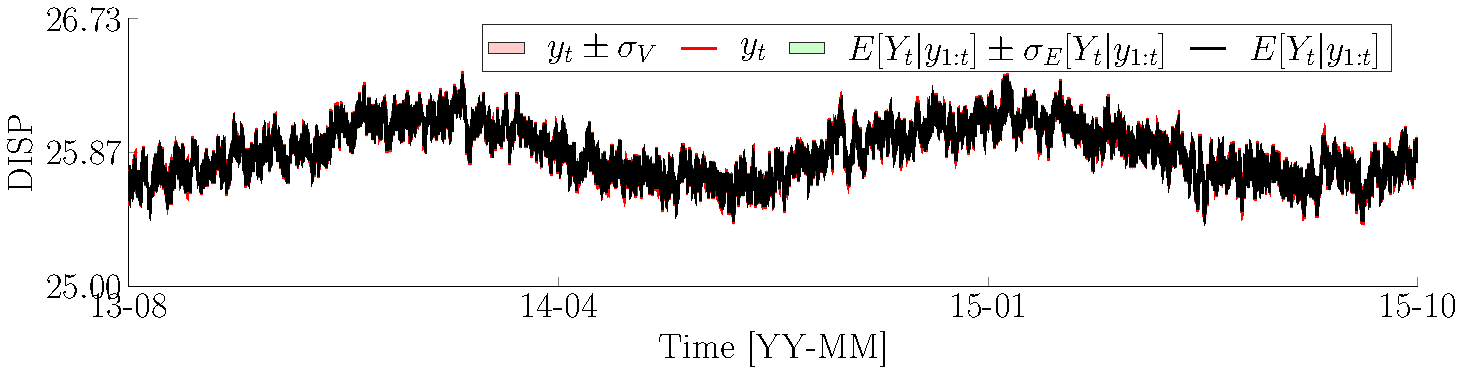
\includegraphics[width=0.9\linewidth]{./docfigs/Example_DISPSIM/default/DISP_ObservedPredicted.pdf} 
%\caption{Observed and estimated displacement data}
%\end{subfigure}
%\begin{subfigure}{\linewidth}
%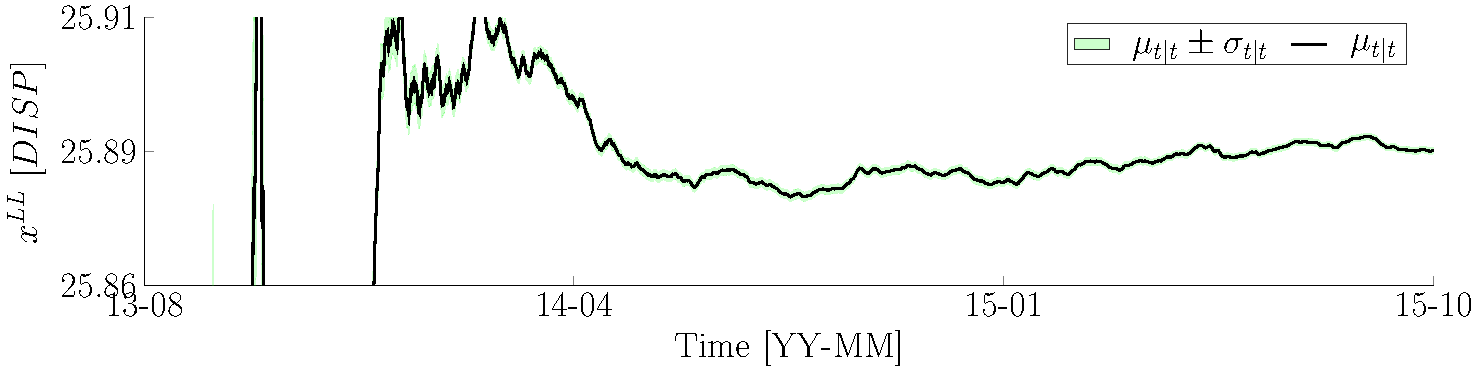
\includegraphics[width=0.9\linewidth]{./docfigs/Example_DISPSIM/default/DISP_LL_1.pdf}
%\caption{Estimated displacement local level component}.
%\end{subfigure}
%\begin{subfigure}{\linewidth}
%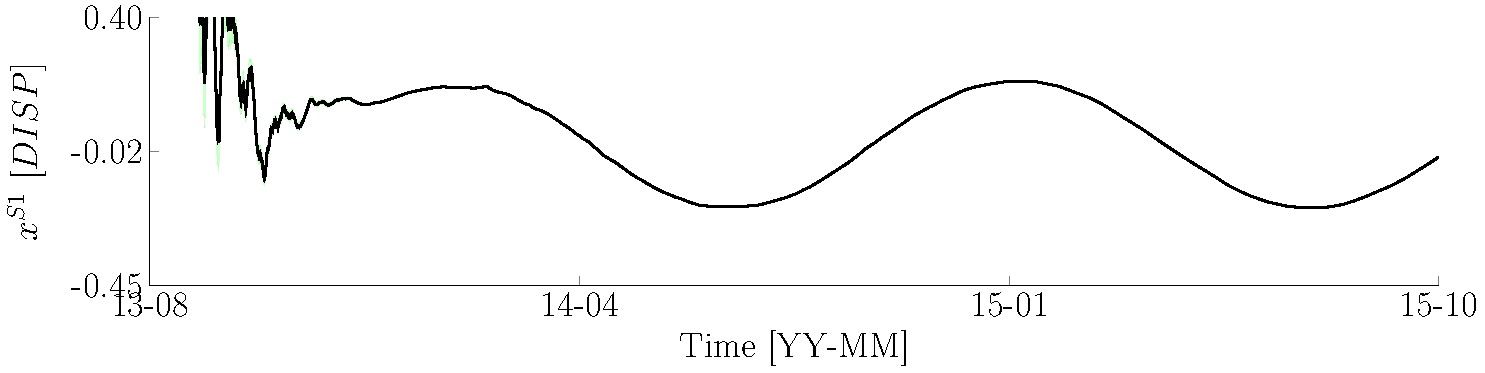
\includegraphics[width=0.9\linewidth]{./docfigs/Example_DISPSIM/default/DISP_S1_2.pdf}
%\caption{Estimated displacement yearly periodic component}
%\end{subfigure}
%\begin{subfigure}{\linewidth}
%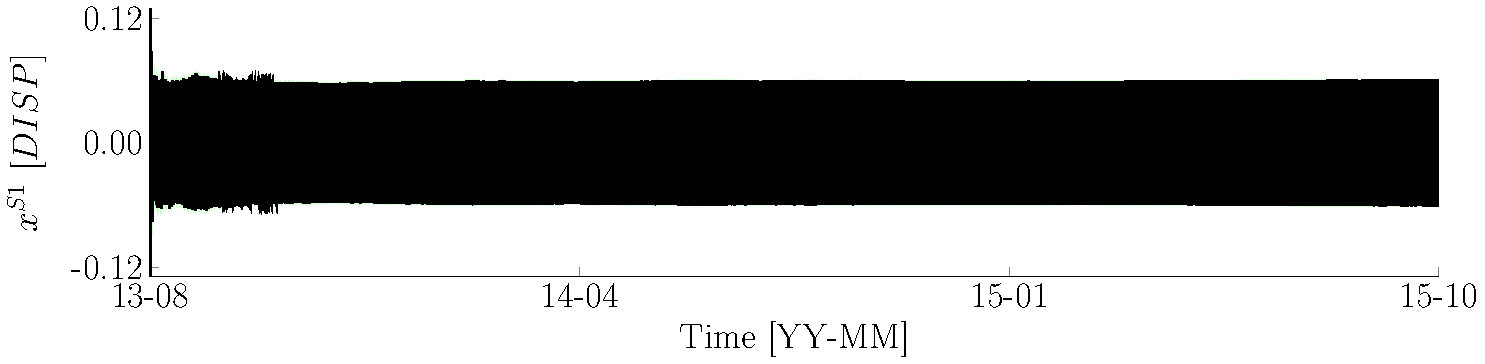
\includegraphics[width=0.9\linewidth]{./docfigs/Example_DISPSIM/default/DISP_S1_4.pdf}
%\caption{Estimated displacement daily periodic component}
%\end{subfigure}
%\begin{subfigure}{\linewidth}
%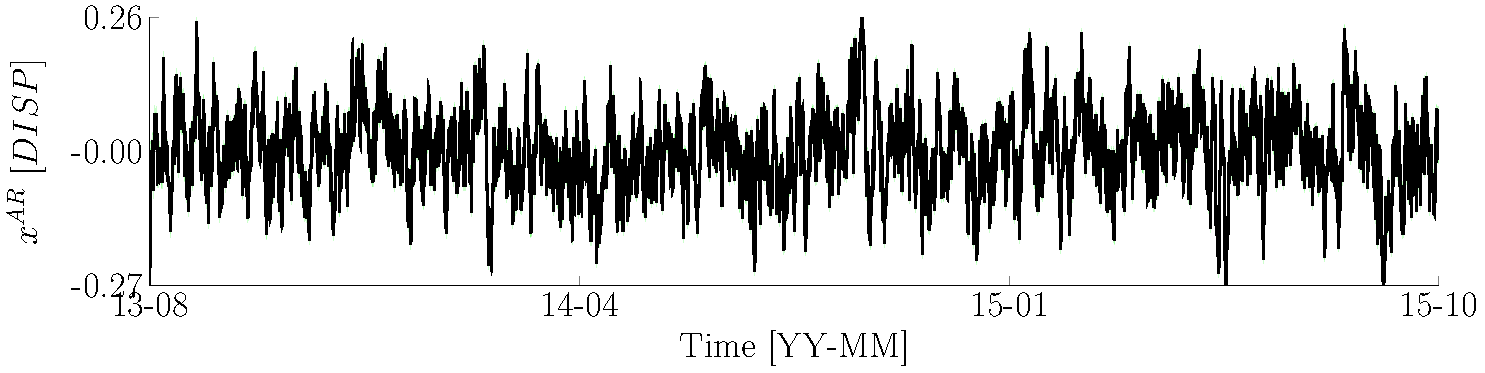
\includegraphics[width=0.9\linewidth]{./docfigs/Example_DISPSIM/default/DISP_AR_6.pdf} 
%\caption{Estimated displacement autoregressive component}
%\end{subfigure}
%\caption{Estimated results using OpenBDLM defaults model parameters and default initial hidden states. The hidden states are estimated from the data presented in Figure~\ref{fig:DataSummary1}a. The solid line and shaded area represent the mean and standard deviation of the estimated hidden states, respectively.}
%\label{fig:Example_DISPSIMDefaultDefaultExample1}
%\end{figure*}
%
%\subsection{Step 7: estimate the model parameters from the data}
%
%Type \colorbox{light-gray}{\lstinline[basicstyle = \mlttfamily \small, backgroundcolor = \color{light-gray}]!OpenBDLM_main('CFG_Example_DISP.m');!} in the \MATLAB{} command line.
%Once, the main menu appears, type  \colorbox{light-gray}{\lstinline[basicstyle = \mlttfamily \small, backgroundcolor = \color{light-gray}]!1!}, then \colorbox{light-gray}{\lstinline[basicstyle = \mlttfamily \small, backgroundcolor = \color{light-gray}]!1!} to estimate the model parameters using Newton-Raphson (type  \colorbox{light-gray}{\lstinline[basicstyle = \mlttfamily \small, backgroundcolor = \color{light-gray}]!2!} to use the Stochastic Gradient Descent instead).
%The model parameters learning procedure starts, and messages are printed on \MATLAB{} command window to monitor the convergence through iterations (see Listing~\ref{LST:OpenBLDMModelParameterLearning}).
%Note that, by default, OpenBDLM considers that the parameters $\sigma_{w}^{LL}$, $p^{\text{PD1}}$, $\sigma_{w}^{\text{PD1}}$ , $p^{\text{PD2}}$, $\sigma_{w}^{\text{PD2}}$ are known.
%Therefore, there are three model parameters to be learned from the data in this example.
%The estimation of the model parameters may take several hours.
%Therefore, press combinations \colorbox{light-gray}{\lstinline[basicstyle = \mlttfamily \small, backgroundcolor = \color{light-gray}]!Ctrl!} + \colorbox{light-gray}{\lstinline[basicstyle = \mlttfamily \small, backgroundcolor = \color{light-gray}]!c!} to abort the process.
%Once the algorithm is converged, the optimized model parameters values should be close to \footnote{Note that it is possible to get slightly different value of parameters with the same performance.}
%\begin{gather*}
%\bm\theta^{\text{*}}=\{0, 365.2422, 0, 1, 0, 0.97, 0.0192, 7.4258\times10^{-7} \}.
%\end{gather*}
%
%\subsection{Step 8: estimate the hidden states using the optimized model parameters values}
%
%In the ``examples/Example\_DISP'' folder, there is a configuration file named \lstinline[basicstyle = \mlttfamily \small, backgroundcolor = \color{light-gray}]!CFG_Example_DISP_optim.m'! that contains optimized model parameters estimated using the Newton-Raphson algorithm.
%Copy and paste \lstinline[basicstyle = \mlttfamily \small, backgroundcolor = \color{light-gray}]!CFG_Example_DISP_optim.m'! from  the ``examples/Example\_DISP'' subfolder  to the ``config\_files'' folder.
%Type \colorbox{light-gray}{\lstinline[basicstyle = \mlttfamily \small, backgroundcolor = \color{light-gray}]!OpenBDLM_main('CFG_Example_DISP_optim.m');!} in the \MATLAB{} command line to load the configuration file  \lstinline[basicstyle = \mlttfamily \small, backgroundcolor = \color{light-gray}]!CFG_Example_DISP_optim.m!.
%Once the main menu appears, type  \colorbox{light-gray}{\lstinline[basicstyle = \mlttfamily \small, backgroundcolor = \color{light-gray}]!3!}, then \colorbox{light-gray}{\lstinline[basicstyle = \mlttfamily \small, backgroundcolor = \color{light-gray}]!1!} to estimate the filtered hidden states using the optimized model parameters and default initial hidden states values.
%The value of the log-likelihood is now $48819$.
%The estimated hidden states are presented in Figure~\ref{fig:Example_DISPSIMOptimizedDefaultExample1}.
%
%\begin{figure*}[h!]
%\begin{center}
%\begin{subfigure}{\linewidth}
%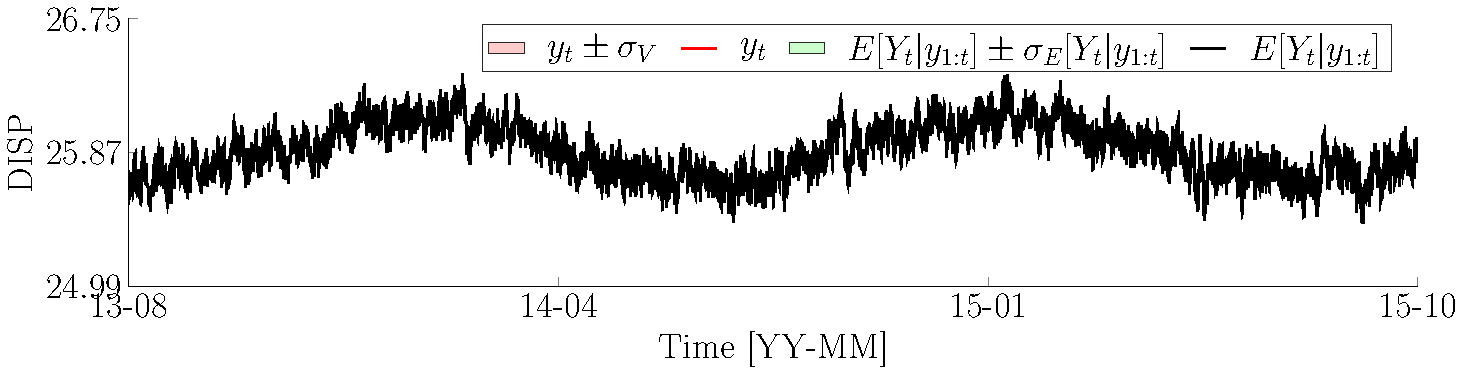
\includegraphics[width=0.9\linewidth]{./docfigs/Example_DISPSIM/optim_param_default_initialhiddenstate/DISP_ObservedPredicted.pdf}
%\caption{Observed and estimated displacement data}
%\end{subfigure}
%\begin{subfigure}{\linewidth}
%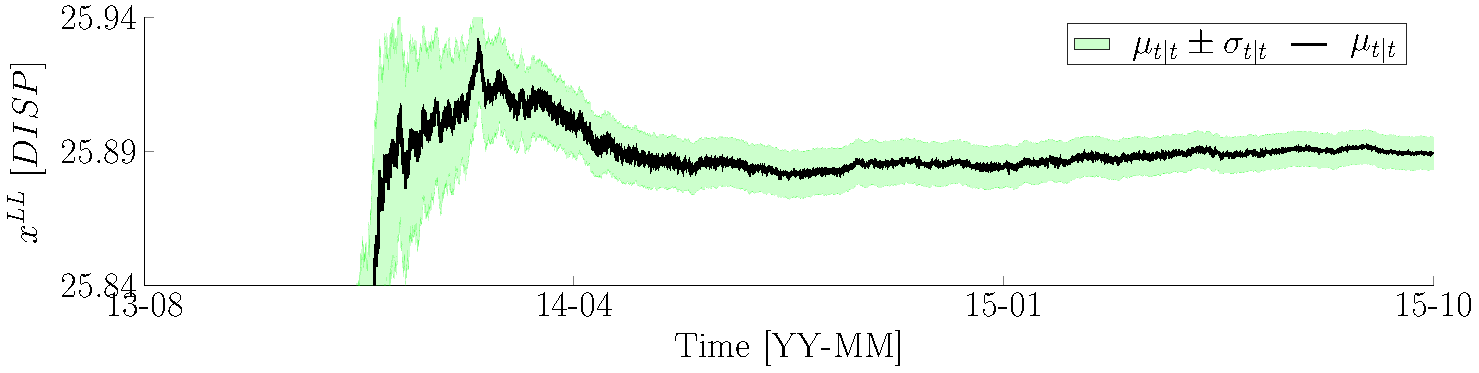
\includegraphics[width=0.9\linewidth]{./docfigs/Example_DISPSIM/optim_param_default_initialhiddenstate/DISP_LL_1.pdf}
%\caption{Estimated displacement local level.}
%\end{subfigure}
%\begin{subfigure}{\linewidth}
%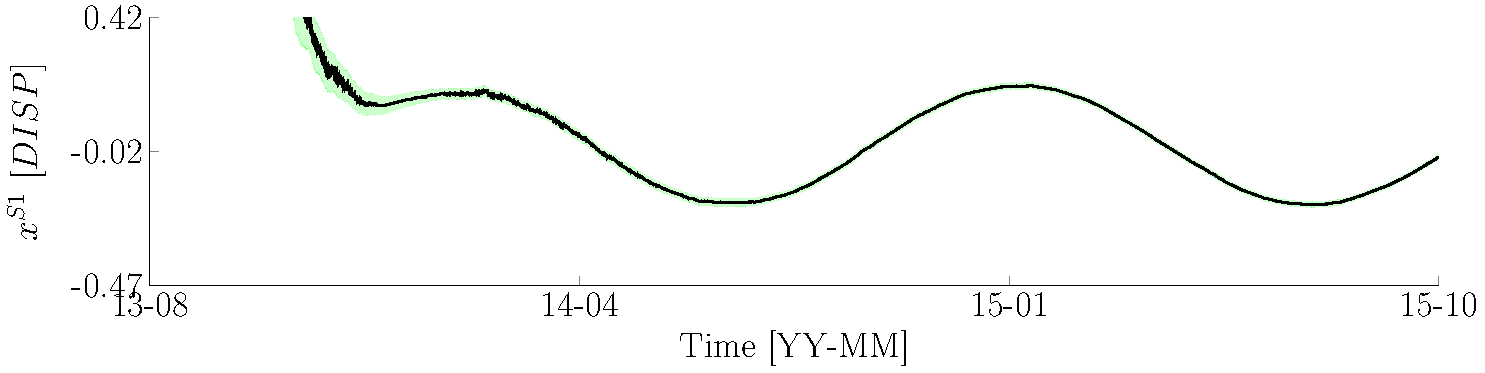
\includegraphics[width=0.9\linewidth]{./docfigs/Example_DISPSIM/optim_param_default_initialhiddenstate/DISP_S1_2.pdf}
%\caption{Estimated displacement yearly periodic component (first hidden state)}
%\end{subfigure}
%\begin{subfigure}{\linewidth}
%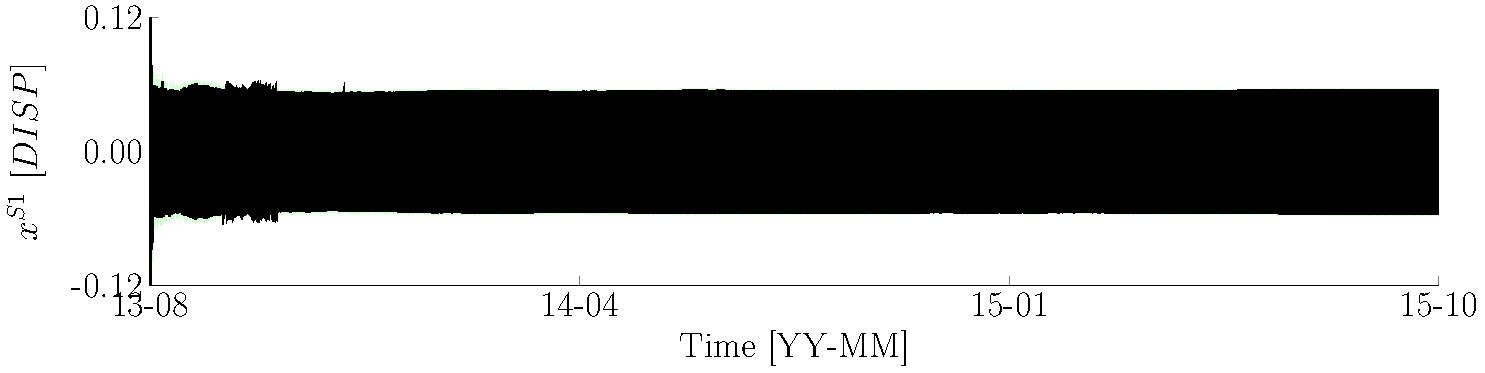
\includegraphics[width=0.9\linewidth]{./docfigs/Example_DISPSIM/optim_param_default_initialhiddenstate/DISP_S1_4.pdf} 
%\caption{Estimated displacement daily periodic component (first hidden state)}
%\end{subfigure}
%\begin{subfigure}{\linewidth}
%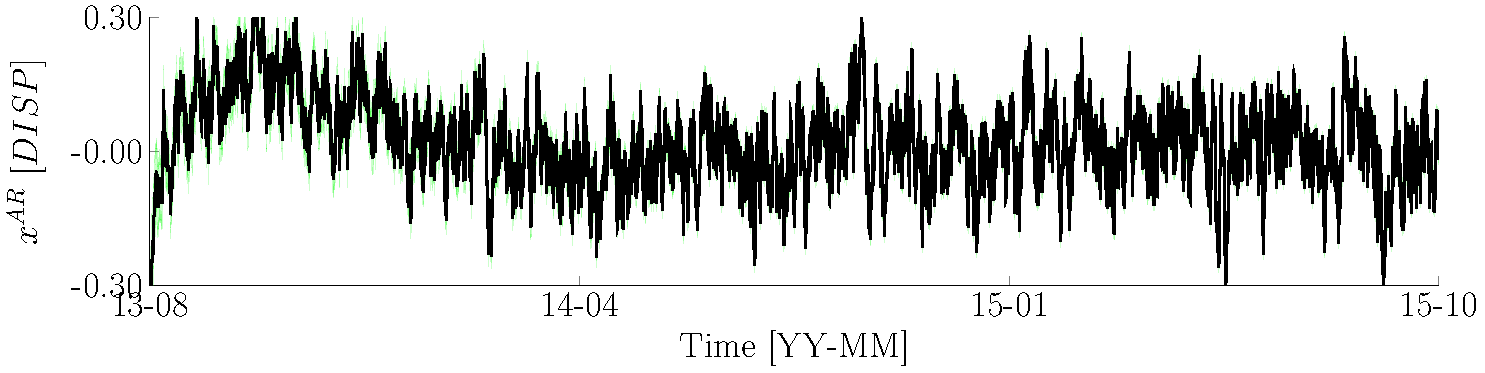
\includegraphics[width=0.9\linewidth]{./docfigs/Example_DISPSIM/optim_param_default_initialhiddenstate/DISP_AR_6.pdf} 
%\caption{Estimated displacement autoregressive component}
%\end{subfigure}
%\caption{Estimated results using OpenBDLM optimized model parameters and default initial hidden states. The hidden states are estimated from the data presented in Figure~\ref{fig:DataSummary1}a. The solid line and shaded area represent the mean and standard deviation of the estimated hidden states, respectively.}
%\label{fig:Example_DISPSIMOptimizedDefaultExample1}
%\end{center}
%\end{figure*}
%
%\subsection{Step 9: estimate the initial hidden states}
%
%Type \colorbox{light-gray}{\lstinline[basicstyle = \mlttfamily \small, backgroundcolor = \color{light-gray}]!OpenBDLM_main('CFG_Example_DISP_optim.m');!} in the \MATLAB{} command line.
%Then, type  \colorbox{light-gray}{\lstinline[basicstyle = \mlttfamily \small, backgroundcolor = \color{light-gray}]!2!}, to optimize the initial hidden states value.
%The estimated initial hidden states mean and covariance values are 
%\begin{align*}
%\bm \mu^{*}_{0} & = [	25.9  ,	-0.204,	-0.00288 ,	0.0341,	0.0521	, -0.0436  ]^{\intercal}, \text{and} \\
% \text{diag}(\bm\Sigma^{*}_{0}) & = [	3.74\times10^{-5} ,	6.87\times10^{-5}	, 7\times10^{-5} , 5.73\times10^{-7} ,	5.73\times10^{-7} , \\
% & 	0.000493    ], 
% \end{align*}
% respectively.
%Once it is done, type  \colorbox{light-gray}{\lstinline[basicstyle = \mlttfamily \small, backgroundcolor = \color{light-gray}]!3!}, and then  \colorbox{light-gray}{\lstinline[basicstyle = \mlttfamily \small, backgroundcolor = \color{light-gray}]!1!} to compute the filtered hidden states using the optimized model parameters and optimized initial hidden states.
%The value of the log-likelihood is $49056$.
%The estimated hidden states are presented in Figure~\ref{fig:Example_DISPSIMOptimizedOptimizedExample1}.


%\begin{figure*}[h]
%\begin{center}
%\begin{subfigure}{\linewidth}
%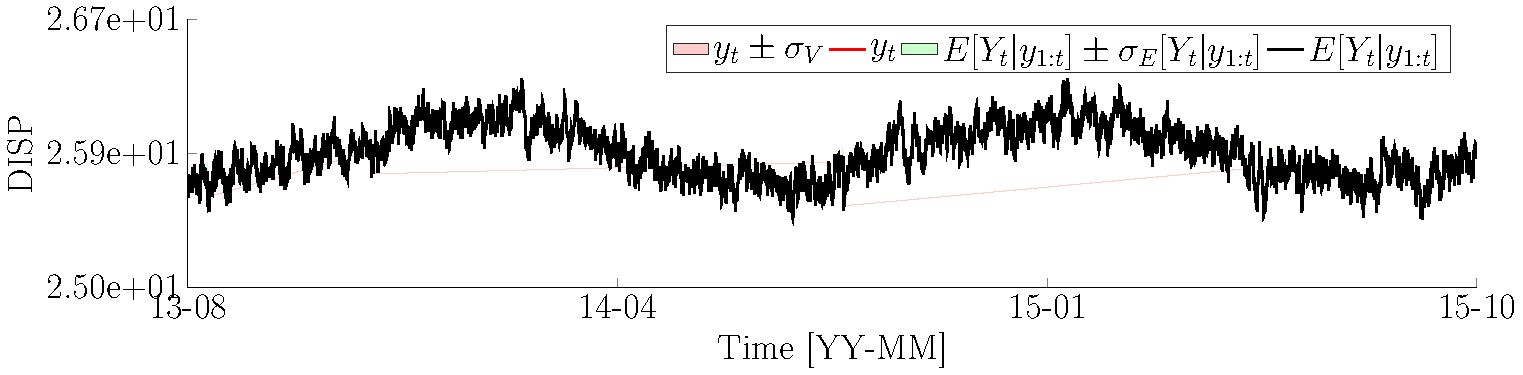
\includegraphics[width=0.9\linewidth]{./docfigs/Example_DISPSIM/optim_param_optim_initialhiddenstate/DISP_ObservedPredicted.pdf} 
%\caption{Observed and estimated displacement data}
%\end{subfigure}
%\begin{subfigure}{\linewidth}
%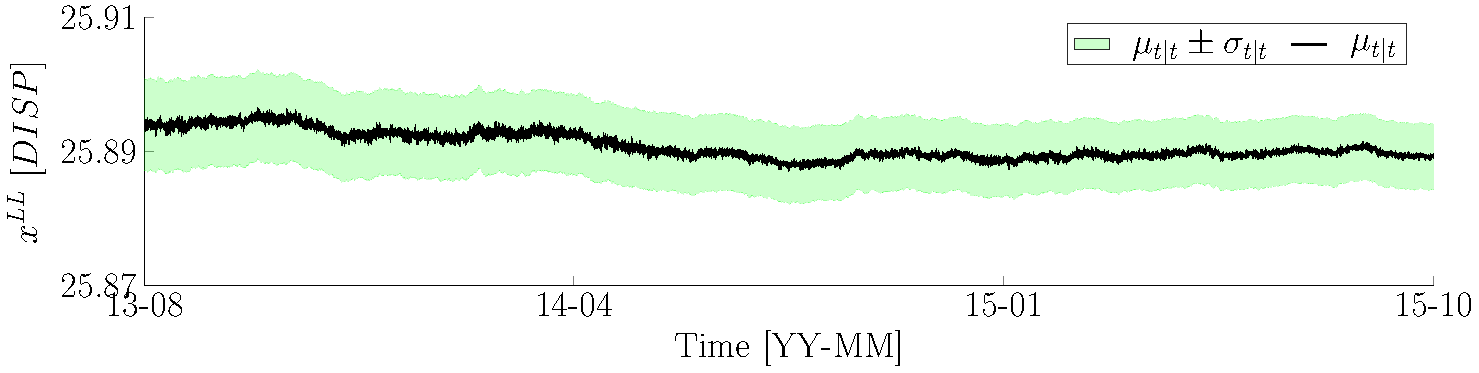
\includegraphics[width=0.9\linewidth]{./docfigs/Example_DISPSIM/optim_param_optim_initialhiddenstate/DISP_LL_1.pdf}
%\caption{Estimated displacement local level component.}
%\end{subfigure}
%\begin{subfigure}{\linewidth}
%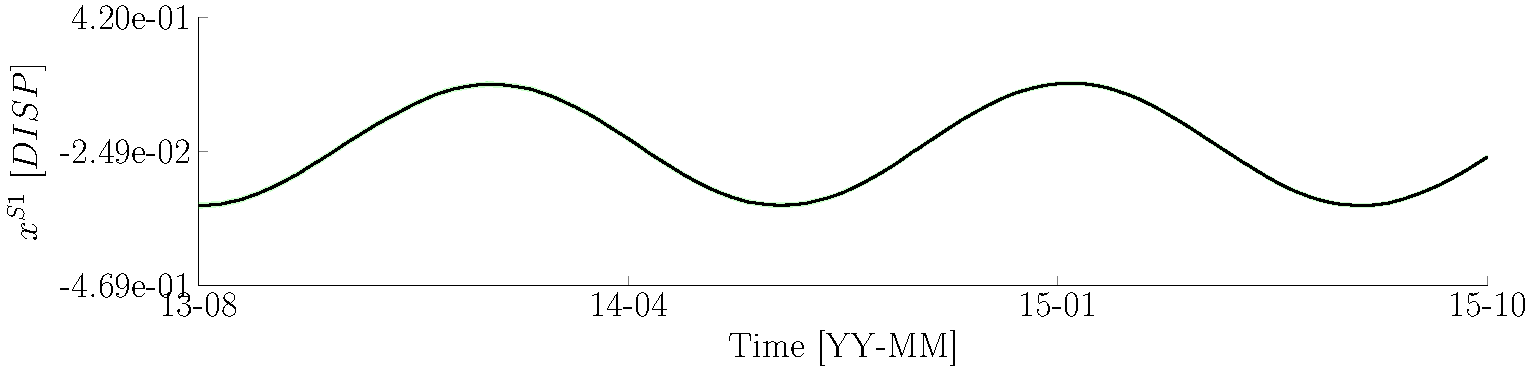
\includegraphics[width=0.9\linewidth]{./docfigs/Example_DISPSIM/optim_param_optim_initialhiddenstate/DISP_S1_2.pdf} 
%\caption{Estimated displacement yearly periodic component (first hidden state)}
%\end{subfigure}
%\begin{subfigure}{\linewidth}
%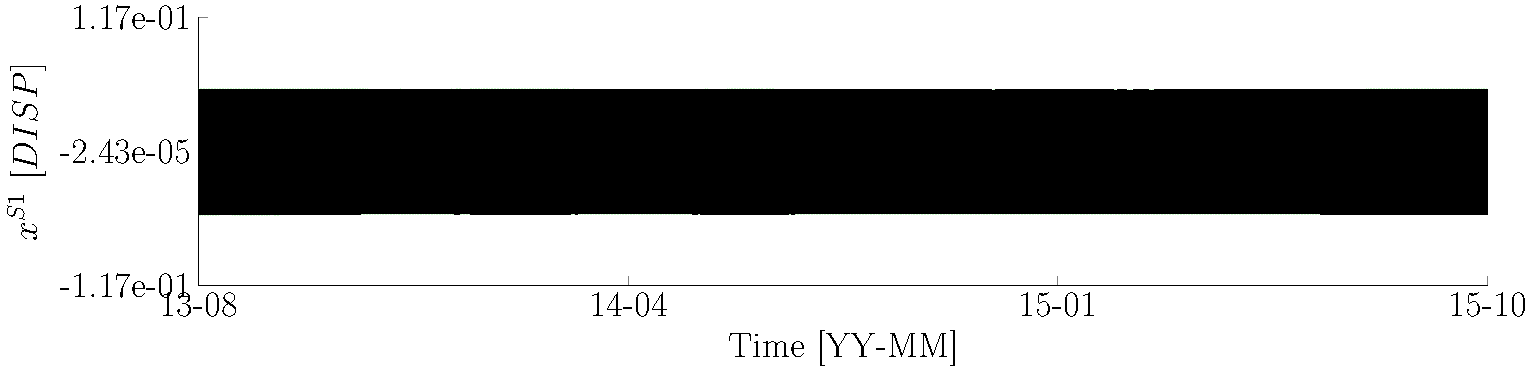
\includegraphics[width=0.9\linewidth]{./docfigs/Example_DISPSIM/optim_param_optim_initialhiddenstate/DISP_S1_4.pdf}
%\caption{Estimated displacement daily periodic component (first hidden state)}
%\end{subfigure}
%\begin{subfigure}{\linewidth}
%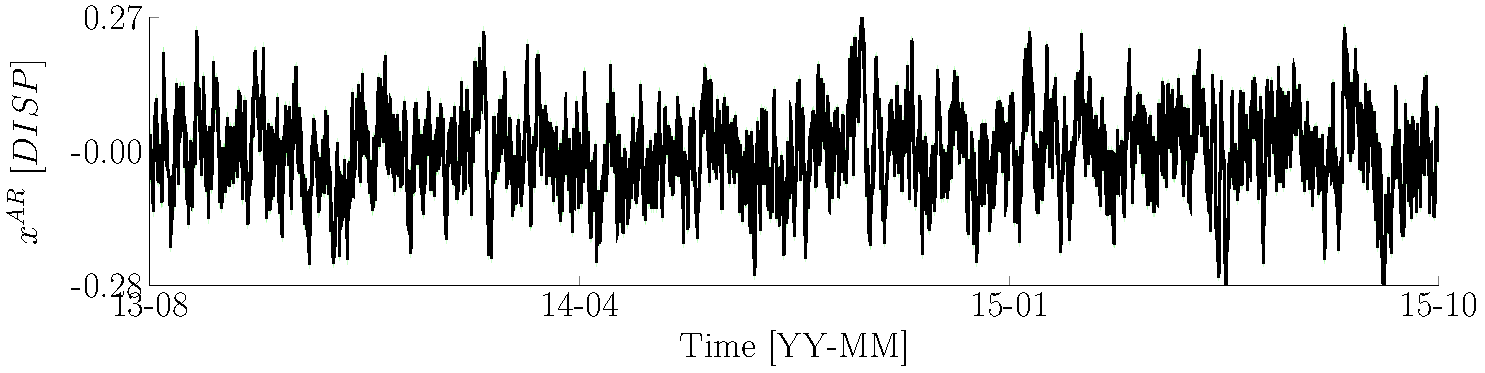
\includegraphics[width=0.9\linewidth]{./docfigs/Example_DISPSIM/optim_param_optim_initialhiddenstate/DISP_AR_6.pdf} 
%\caption{Estimated displacement autoregressive component}
%\end{subfigure}
%\caption{Estimated results using OpenBDLM optimized model parameters and optimized initial hidden states. The hidden states are estimated from the data presented in Figure~\ref{fig:DataSummary1}a. The solid line and shaded area represent the mean and standard deviation of the estimated hidden states, respectively.}
%\label{fig:Example_DISPSIMOptimizedOptimizedExample1}
%\end{center}
%\end{figure*}


%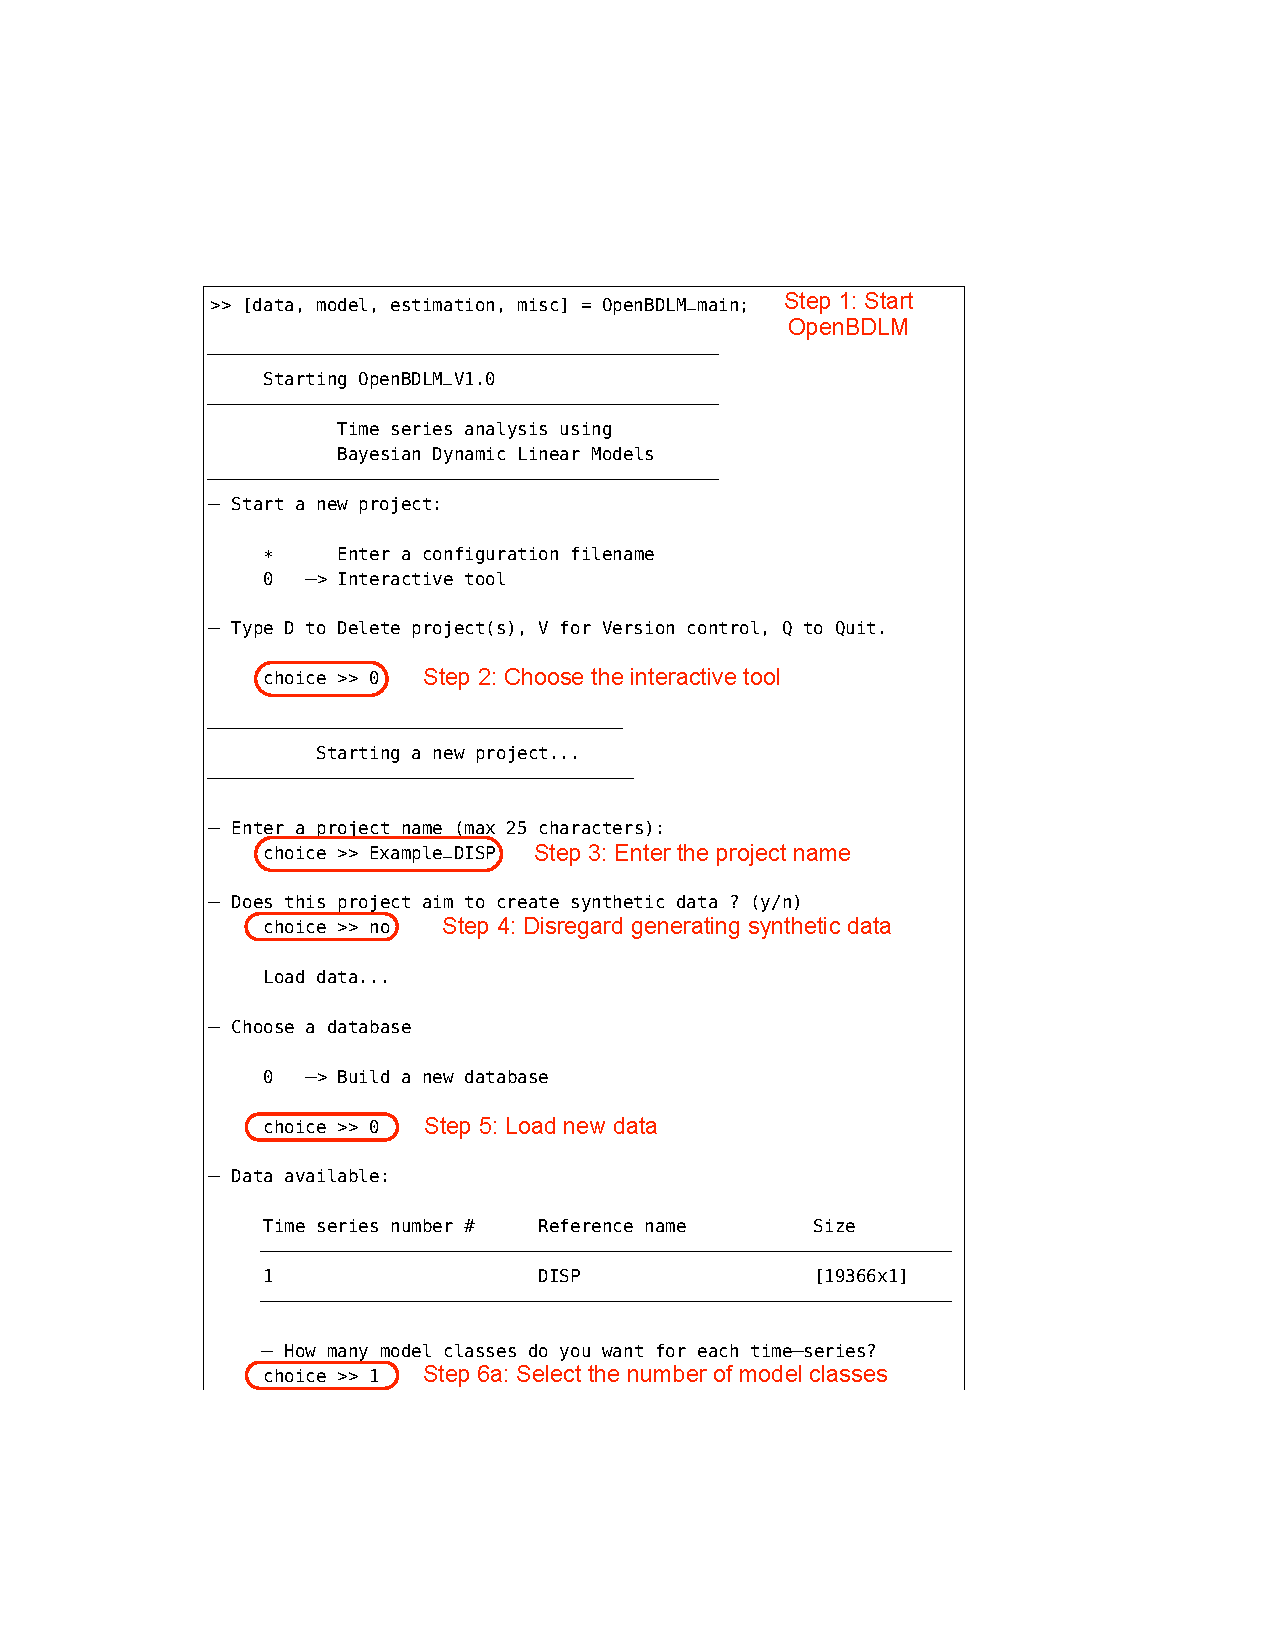
\includepdf[pages=-, pagecommand={\thispagestyle{plain}}]{./docfigs/Example_DISPSIM/listing/listing_step_by_step_2.pdf}

